\subsection{Kernel Treiber}

\begin{wrapfigure}[23]{o}[1cm]{8cm}
\dirtree{%
.1 /.
.2 install\_driver.sh.
.2 .gitignore.
.2 README.md.
.2 doc/.
.2 app/.
.2 driver/.
.3 Makefile.
.3 spidev\_disabler.dts.
.3 src/.
.4 fanctrl.c.
.4 fanctrl.h.
.4 fops.c.
.4 fops.h.
.4 pwm.c.
.4 pwm.h.
.4 temp.c.
.4 temp.h.
.4 ioctl.c.
.4 ioctl.h.
}
\caption{Ordnerstruktur des Treibers}
\label{fig:driverdirectory}
\end{wrapfigure}

Der Code des Kernel-Treibers ist in \texttt{C99} geschrieben.
Dieser ist Prozessoragnostisch.
Es werden jedoch existierende low-level Treiber zwischen den Prozessorregistern und Kerenlspace erwartet, die die Kommunikation über \gls{i2c} und \gls{spi} abstrahieren.
Das Modul an sich ist lediglich von linux-Headern abhängig.
Der Treiber ist auf verschiedene \texttt{C}-Dateien aufgeteilt.
Die Struktur des Treibers ist in \autoref{fig:driverdirectory} aufgeführt.
Der Tatsächliche Quellcode für den Treiber befindet sich lediglich im \texttt{src} Ordner.
Alle anderen Dateien sind notwendig jedoch kein direkter Teil des Treibers.

Die Haupt-Datei mit dem Anfangspunkt des Treibers ist in \texttt{fanctrl.c}.
Darin wird das Treibermodul initialisiert, registriert, ausgeführt und schließlich auch de-initialisiert.
Der Kernel-Treiber kann über sowohl durch \gls{fops} als auch mit \gls{ioctl} mit dem Userspace kommunizieren.
Dies wird in den \texttt{fops.c} und \texttt{ioctl.c} und deren jehweils dazugehörigen Header-Files implementiert.
Die anderen zwei Hauptfunktionen, die Kommunikation über \gls{i2c} und \gls{spi} werden in \texttt{temp.c} und \texttt{pwm.c} respektiv implementiert.
In den folgenden Abschnitten werden die implementierten Funktionen, zusätzliche Dateien und der Kompilierungs/Installationsvorgang beschreiben.

\subsubsection{Temperatursensor über \acrshort{i2c}}

Mit der Funktion \texttt{void tempInit(void)} in \autoref{code:i2c-init} wird der \gls{i2c} Adapter initialisiert.
Dannach wird ein neuer \gls{i2c} Device hinzugefügt und der Treiber wird dem Adapter registriert.
Der Device beinhält die Informationen über Device Name und Addresse.
Ist der Adapter initialisiert wird dieser mit \texttt{void tempDeinit(void)} in \label{code:i2c-deinit} zum Programm Ende, falls er erfolgreich initialisiert wurde, wieder deinitialisiert.
Dabei werden alle vom \gls{i2c} Adapter genutzen Ressourcen für den Treiber frei gegeben.
Auf dem \gls{rpi} muss \gls{i2c} durch die \texttt{raspi-config} aktiviert werden.

\lstinputlisting[firstnumber=17, firstline=17,lastline=27, language=C, caption={\texttt{./driver/src/temp.c:17-27}}, label=code:i2c-init, float=b]{../../driver/src/temp.c}

\lstinputlisting[firstnumber=29, firstline=29,lastline=34, language=C, caption={\texttt{./driver/src/temp.c:29-34}}, label=code:i2c-deinit, float=b]{../../driver/src/temp.c}

Der \texttt{TMP102} Sensor gibt Messdaten mit 13-Bit Präzision bei einer Auflösung von $0.0625\si{\degree C}$ am \gls{lsb} an.
Um einen Messwert zu einer Temperatur zu konvertieren müssen zuerst zwei Byte gelesen werden.
Diese müssen zu einem 16-Bit Wert, welcher den ogrinellen 13-Bit Messwert beinhaltet, konkatiniert werden.
Anschlie{\ss}end muss der Messwert linear abgebildet werden, dass hei{\ss}t mit der Auflösung pro \gls{lsb} multiplizieren.
Die \gls{fpu} sollte unter allen Umständen nicht aus dem Kernelspace verwendet werden,
da die Kontextänderung abträgliche Performanceimplikationen auf Userspace Applikationen mit sich führen kann.
Die berechnung wird folglich mit der Integerdivision des Kehrwerts wie in \autoref{eq:temp-convert} ausgeführt.
Der Fehler der Berechnung wird in \autoref{eq:temp-error} aufgeführt und in \autoref{fig:rounding-err} visualisiert.
Der resultierende Rundungsfehler manifestiert sich als Rauschen.
Da unsere Anwednung sich nominal bei und über Raumtemperatur in Einer-Stellen Präzision agiert sind die resultierenden Fehler vernachlässigbar.
Die Implementation der Kommunikation mit dem Sensor und Wandlung der Daten ist in \autoref{code:i2c-convert} gegeben.

\begin{equation}
    \vartheta = \texttt{M}_D \cdot 0.0625\si{\celsius} = \frac{\texttt{M}_D}{\left(0.0625\si{\celsius}\right)^{-1}} = \frac{\texttt{M}_D}{16\si{\per\celsius}} \approx \left\lfloor\frac{\texttt{M}_D}{16\si{\per\celsius}}\right\rfloor
    \label{eq:temp-convert}
\end{equation}
\begin{equation}
    \begin{aligned}
        \Delta_{\texttt{M}_D} &= \frac{\texttt{M}_D}{16\si{\celsius}} - \left\lfloor\frac{\texttt{M}_D}{16\si{\per\celsius}}\right\rfloor \\[2ex]
        \delta_{\texttt{M}_D} &= \frac{\Delta_{\texttt{M}_D}}{\frac{\texttt{M}_D}{16\si{\celsius}} }\\[2ex]
    \end{aligned}
    \label{eq:temp-error}
\end{equation}

\begin{figure}
    \centering
    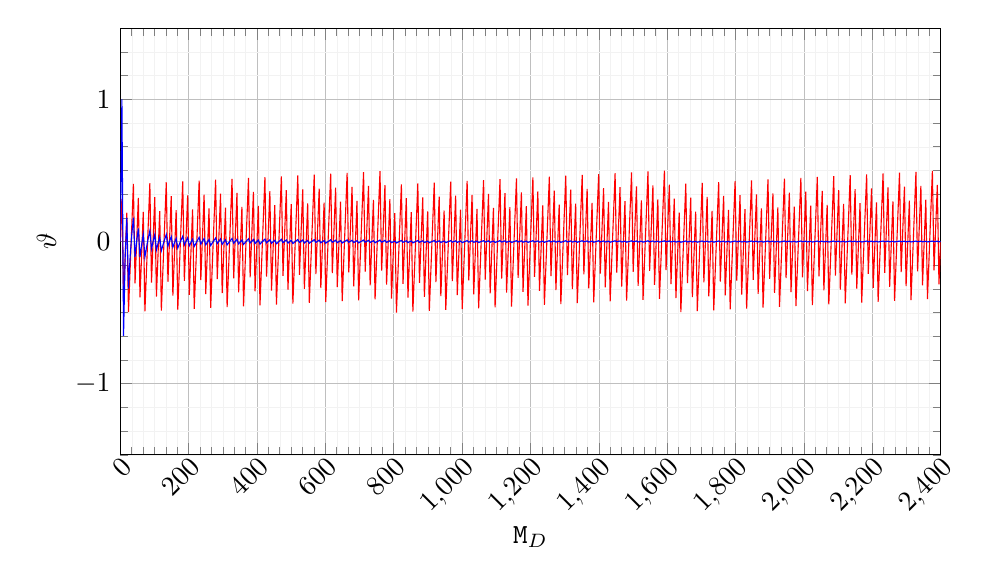
\begin{tikzpicture}
        \begin{axis}[%
            xmin=0,
            xmax=2400,
            ymin=-1.5,
            ymax=1.5,
            samples=500,
            width=12cm,
            height=7cm,
            minor tick num=5,
            grid=both,
            grid style={line width=.1pt, draw=gray!10},
            major grid style={line width=.2pt,draw=gray!50},
            % nodes near coords,
            xlabel near ticks,
            xticklabel style={rotate=45,anchor=north east,inner sep=0mm},
            xlabel={$\texttt{M}_D$},
            ylabel={$\vartheta$},
            ylabel near ticks]
            % \addplot[domain=0:6.4, blue, very thick, smooth, ->] {2.1971*1.8206^x};
            \addplot[domain=0:2400, red] {(x * 0.0625) - round(x / 16)};
            \addplot[domain=0:2400, blue] {((x * 0.0625) - round(x / 16)) / (x * 0.0625)};
        \end{axis}
    \end{tikzpicture}
    \caption[Integerdivisionsinduzierter Rundungsfehler]{Integerdivisionsinduzierter Rundungsfehler der Temperatursensorkonversion
    \textcolor{red}{Rot: Absoluter Fehler $\Delta_{\texttt{M}_D}$.}
    \textcolor{blue}{Blau: Relativer Fehler $\delta_{\texttt{M}_D}$.}
    }
    \label{fig:rounding-err}
\end{figure}

\lstinputlisting[firstnumber=37, firstline=37,lastline=49, caption=\texttt{./driver/src/temp.c:37-49}, label=code:i2c-convert, float]{../../driver/src/temp.c}

\subsubsection{Potentiometer über \acrshort{spi}}

\subsubsubsection{Protokoll}

% TODO Beschreiben welche Bits zu dem Potentiometer über SPI geschickt werden

\subsubsubsection{Softwareablauf}

% TODO Beschreibung von Code Abschnitten über SPI

\subsubsubsection{Devicetree Overlay}
Auf dem \gls{rpi} muss der \gls{spi} Treiber durch \texttt{raspi-config} aktiviert werden.
Dadurch werden unter \texttt{/dev} zwei \gls{spi} Treiber angelegt und das Hardware \gls{spi} Subsystem aktiviert.
Die angelegten Treiber stellen eine \gls{api}-Verbindung zwischen Kernelspace und der Hardware dar.
Jedoch werden durch die Treiber die \gls{ss} Signale belegt.
Der Treiber zur Kommunikation über \gls{spi} funktioniert, kann jedoch aufgrund dessen nicht durch externe Programme im Kernelspace beansprucht werden.
Um dies zu umgehen muss der Zugriff auf die \gls{ss} Signale durch die durch das System bereitgestellten Treiber unterbunden werden.

Dazu wird der Devicetree zur Laufzeit mit einem Patch injeziert.
Deswegen stehen die \gls{ss} Signale frei zur Verfügung, um durch unseren Treiber aus dem Kernelspace genutzt zu werden.
Das Devicetree Overlay wird mit dem devicetree compiler kompiliert:
\begin{lstlisting}
dtc spidev_disabler.dts -O dtb < spidev_disabler.dtbo
\end{lstlisting}
Das generierte Overlay wird dannach injeziert:
\begin{lstlisting}
sudo dtoverlay -d . spidev_disabler
\end{lstlisting}

\subsubsection{\acrshort{fops}}

% TODO Beschreiben von FOPS Treiber

\subsubsection{\Acrshort{ioctl}}

% TOOD Beschreiben von IOCTL Treiber

\subsubsection{Kompilierung und Verlinkung}

Der Treiber kann automatisch kompiliert und als Kernel Objekt verlinkt werden.
Danach kann das erstelle Kernel Objekt auch geladen werden.
\begin{lstlisting}
make all
sudo insmod fanctrl.ko
\end{lstlisting}

Um den Entwicklungslebenszyklus zu vereinfachen besteht auch die Möglichkeit den gesamten Zyklus automatisch auszuführen.
Mit dem \texttt{install\_driver.sh} Skript wird das Kernelmodul entladen, neu kompiliert, das Devicetree Overlay neu geladen und das Kernel Modul wieder neu geladen.
